\chapter{State of the Art}
\label{chap2}
% \thispagestyle{fancy}
\textit{This chapter presents a comprehensive review of the literature, evaluating the current advances in the fields and identifying research gaps in the optimal control of soft quadruped robots and the model-based reinforcement learning.}

\section{Robot Control}
Robot can be treated as a machine that is designed to perform tasks automatically and often in a precise way\cite{biswalDevelopmentQuadrupedWalking2021}, so the control of a robot is quite important. The first quadruped robot The control of quadruped robot focuses on various aspects, including locomotion control\cite{dingNovelDynamicLocomotion2020}, balance and stability\cite{sunBalanceControlQuadruped2022}, and gait planning\cite{liGaitPlanningStability2016} among the four legs of robot, since the lower level control of quadruped robot was well studied and tailored for specific applications.

The process of implementing control for a robot involves a hierarchical approach, starting from lower-level mechanisms controls and gradually progressing to higher-level task-specific behaviors. At the lower level, motor control is achieved by developing firmware or low-level code to facilitate precise manipulation of actuators, enabling control over essential parameters such as speed, direction, and torque. Sensor integration plays a vital role, as it allows the robot to perceive its environment and gather crucial feedback. This integration encompasses various sensors, such as encoders for motor position tracking, inertial measurement units for orientation and acceleration measurements, proximity sensors for obstacle detection, and cameras for visual perception. Leveraging this sensor data, feedback control loops are implemented to regulate and fine-tune the robot's behavior. To account for the robot's mechanical structure, kinematics and dynamics principles are applied, allowing for precise control considering factors such as joint angles, leg positions, and forces exerted on the system. Trajectory planning techniques come into play to generate smooth and feasible paths for the robot's motion, considering task requirements and constraints. State estimation and localization algorithms provide accurate and reliable estimates of the robot's position, orientation, and velocity by fusing sensor data and utilizing filtering methods. Finally, task-specific control strategies are implemented, tailoring the robot's behaviors to accomplish specific objectives. This may involve higher-level control algorithms, including behavior-based control, hierarchical control, or planning algorithms, designed to address complex tasks such as obstacle avoidance, goal-seeking, or path planning. The comprehensive understanding and systematic implementation of these control mechanisms enable the development of robotic systems capable of precise and adaptive control in diverse environments and applications.

\subsection{Kinematics}
Kinematics refers to the study of the geometric properties of motion without considering the forces or torques involved. In the case of quadruped robots, kinematics focuses on determining the relationships between joint angles, leg positions, and the resulting end-effector positions and orientations. By understanding the kinematics of the robot, one can compute the desired joint angles or leg positions required to achieve specific end-effector poses. Kinematic models are often represented through geometric transformations, such as homogeneous transformations or Denavit-Hartenberg parameters, which describe the relative positions and orientations of different robot links.

Dynamics, on the other hand, involves the study of the forces and torques that influence the robot's motion. In the context of quadruped robots, dynamics principles help in understanding how the forces and torques at each joint and leg affect the overall motion and stability of the robot. Dynamic modeling involves considering factors such as mass, inertia, friction, and external forces acting on the robot. By modeling the dynamics of the system, one can accurately predict the forces and torques required to achieve desired motions or maintain balance.

Furthermore, kinematic and dynamic analysis assist in optimizing the control strategies for quadruped robots. By analyzing the robot's kinematic and dynamic properties, it becomes possible to identify optimal gait patterns, joint coordination strategies, or control parameters that enhance stability, locomotion efficiency, and task performance. These principles also contribute to the development of advanced control algorithms, such as model-based control or optimization-based control, which utilize kinematic and dynamic models to optimize control signals and achieve desired performance objectives.

\subsection{Gait Controller}
The gait controller is a kind of scheduler. 

The integration of advanced control mechanisms, as discussed above, serves as a solid foundation for the introduction of robot learning into the control framework. While control algorithms provide a means to govern robot behavior, robot learning complements this by enabling robots to acquire knowledge and improve their control strategies through experience and interaction with the environment. By incorporating machine learning techniques, robots can go beyond pre-programmed behaviors and adapt their control policies based on real-time sensory information and learned models. Robot learning empowers robots to autonomously acquire new skills, optimize their performance, and adapt to novel situations, thereby enhancing their adaptability, flexibility, and efficiency. By combining the principles of robust control with the capabilities of robot learning, the field of robotics is continually advancing towards developing intelligent and adaptive systems that can autonomously learn, adapt, and perform complex tasks in dynamic and uncertain environments.

The field of robot control has made significant advancements in achieving precise and efficient task execution, balance, and stability in robots. However, to further enhance the capabilities of robotic systems, researchers have recognized the importance of integrating robot learning into the control framework. By introducing robot learning, robots can go beyond pre-programmed behaviors and adapt their control strategies based on real-time sensory information and interactions with the environment. Robot learning empowers robots to acquire new skills, optimize their performance, and handle complex and uncertain situations with greater autonomy. By combining the principles of robot control with the capabilities of robot learning, the field of robotics continues to push the boundaries of what robots can achieve, opening up exciting possibilities for applications in diverse domains such as manufacturing, healthcare, and exploration.

\subsection{Trajectory Control}
Controlling the trajectory of a quadruped robot entails the precise coordination of leg movements to achieve desired locomotion patterns and effective navigation within its environment. Trajectory control in quadruped robots concentrates on factors such as locomotion stability, balance, and optimized gait patterns. To accomplish this, a trajectory planning process is initiated by defining the desired trajectory, encompassing parameters such as the robot's position, orientation, and velocity at different time instances, with task-specific requirements dictating the trajectory's characteristics.

To achieve the intended trajectory, a variety of control techniques are employed. These techniques encompass the generation of leg motions and coordination strategies. Key techniques include gait planning, which determines the optimal sequencing and timing of leg movements to achieve stable locomotion by specifying the instances of leg-ground contact. Inverse kinematics calculations are utilized to deduce the necessary joint angles or leg positions that correspond to desired end-effector positions. By addressing the inverse kinematics problem, the control system can generate leg trajectories that align with the desired trajectory.

Dynamic balance control is crucial for quadruped robots to maintain stability during locomotion and mitigate the risk of falls or instability. This entails adjusting leg forces and positions in response to variations in the robot's center of mass or external disturbances. Moreover, terrain adaptation techniques are implemented to cater to the complex and uneven terrains in which quadruped robots often operate. These techniques involve modifying leg motions, forces, or joint angles to accommodate changes in ground height, slope, or roughness, ensuring stable locomotion and trajectory adherence.
\subsection{Model Predictive Control}


\section{Robot Learning}
Robot learning refers to the ability of a robot to acquire knowledge and improve its performance through experience, interaction with the environment, and data-driven methods. It involves enabling robots to learn from their own actions, from human guidance, or from analyzing large amounts of data. The goal of robot learning is to equip robots with the ability to adapt, generalize, and improve their behavior over time without being explicitly programmed for every possible scenario.

Robot learning can encompass various techniques, including machine learning, reinforcement learning, imitation learning, and deep learning. These techniques enable robots to acquire new skills, optimize their performance, and adapt to changing conditions. By leveraging data from sensors, feedback from humans, or interactions with the environment, robots can learn to perceive and understand their surroundings, make informed decisions, and execute tasks more effectively.

Machine learning algorithms allow robots to extract meaningful patterns and information from data, enabling them to recognize objects, navigate environments, and perform complex tasks. Reinforcement learning involves training robots through a trial-and-error process, where they receive feedback or rewards for their actions, allowing them to learn optimal strategies. Imitation learning enables robots to learn by observing and imitating human demonstrations. Deep learning techniques, such as neural networks, provide the ability to process and interpret complex sensory data, enabling robots to understand and respond to their environment.


\subsection{Reinforcement Learning}
As the complexity of robotics increases, \ac{RL} is increasingly required to develop robust control algorithms with high \ac{DoF}s and time variant properties\cite{zhangEffectiveSoftRobot2017}. The rapid development of AI provides an alternative solution to take into account the nonlinear properties of novel materials and soft robots\cite{tangModelbasedOnlineLearning2021}. \ac{MFRL} is a type of reinforcement learning where an agent learns to make decisions based on experiences and rewards obtained from the environment, without having an explicit model of the environment. The agent directly can map observations to actions, through trial and error, without considering the underlying dynamics of the environment\cite{arulkumaranDeepReinforcementLearning2017}. The goal of model-free reinforcement learning is to learn a policy $\Pi$, which is a mapping from states to actions, that maximizes the expected cumulative reward over time. The \ac{MBRL} refers to a type of \ac{RL} where an agent learns optimal behavior by learning a model of the environment by taking actions and observing the outcomes that include the next step and the immediate reward\cite{rayModelBasedReinforcementLearning2010}. 
\begin{figure}[hp]
    \centering
    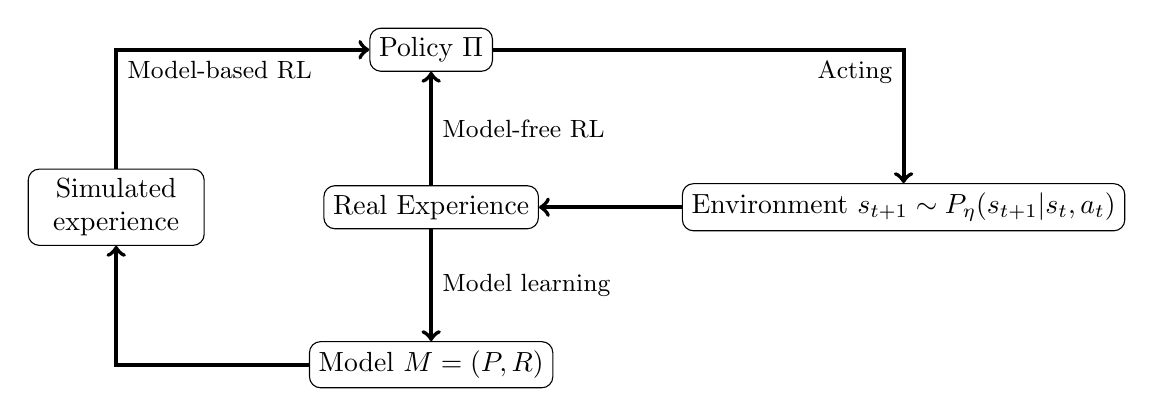
\begin{tikzpicture}[node distance=2cm]
        % Define nodes
        \node (policy) [rounded corners, draw] {Policy $\Pi$};
        \node (real_experience) [rounded corners, draw, below of=policy] {Real Experience};
        \node (environment) [rounded corners, draw, right of=real_experience, node distance=6cm] {Environment $s_{t+1}\sim P_\eta(s_{t+1}|s_t, a_t)$};
        \node (model) [rounded corners, draw, below of=real_experience] {Model $M = (P,R)$};
        \node (simulated_experience) [align=center, text width=2cm, rounded corners, draw, left of=real_experience, node distance=4cm] {Simulated experience};
        
        % Draw arrows
        \draw[->, line width=1.5pt] (policy) -| (environment) node[midway, below left, font=\small] {Acting};
        \draw[->, line width=1.5pt] (environment) -- (real_experience);
        \draw[->, line width=1.5pt] (real_experience) -- (model) node[midway, right, font=\small] {Model learning};
        \draw[->, line width=1.5pt] (model) -| (simulated_experience);
        \draw[->, line width=1.5pt] (real_experience) -- (policy) node[midway, right, font=\small] {Model-free RL};
        \draw[->, line width=1.5pt] (simulated_experience) |- (policy) node[font=\small, midway, below right] {Model-based RL};
    \end{tikzpicture}
    \caption{Model-free \ac{RL} vs. Model-based \ac{RL}}
    \label{fig:demo}
\end{figure}
% \tikzstyle{block} = [draw, fill=white, rectangle, 
%     minimum height=3em, minimum width=6em]
% \tikzstyle{sum} = [draw, fill=white, circle, node distance=1cm]
% \tikzstyle{input} = [coordinate]
% \tikzstyle{output} = [coordinate]
% \tikzstyle{pinstyle} = [pin edge={to-,thin,black}]

% \begin{tikzpicture}[auto, node distance=2cm,>=latex']

%     \node [input, name=input] {};
%     \node [sum, right of=input] (sum) {};
%     \node [block, right of=sum] (controller) {Controller};
%     \node [block, right of=controller, pin={[pinstyle]above:D},
%             node distance=3cm] (system) {System};

%     \draw [->] (controller) -- node[name=u] {$u$} (system);
%     \node [output, right of=system] (output) {};
%     \node [block, below of=u] (measurements) {Measurements};

%     \draw [draw,->] (input) -- node {$r$} (sum);
%     \draw [->] (sum) -- node {$e$} (controller);
%     \draw [->] (system) -- node [name=y] {$y$}(output);
%     \draw [->] (y) |- (measurements);
%     \draw [->] (measurements) -| node[pos=0.99] {$-$} 
%         node [near end] {$y_m$} (sum);
% \end{tikzpicture}


Typically, the model can be considered as a combination of state transition distribution $P_\eta$ and reward function $R_\eta$, $$M = (P,R) \textrm{ where } s_{t+1}\sim P_\eta(s_{t+1}|s_t, a_t) \textrm{ and } r_{t+1}\sim R_\eta(r_{t+1}|s_t, a_t)$$ $s_t$ is the state at time $t$, $r_t$ is the reward at time $t$ and $a_t$ is the action at time $t$. \ac{MBRL} learns an abstract model of the environment to plan the optimal policy. This model can be used to simulate the consequences of its actions, allowing it to make informed decisions, which makes it applicable to handle more complex environments, as it can make use of a model of the environment's dynamics. Therefore, model-based \ac{RL} requires a prior knowledge of the domainology\cite{tangModelbasedOnlineLearning2021}, as a model needs to be created and maintained. The domain of the model-based \ac{RL} refers to the context or environment in which the \ac{RL} agent is operating, which determines the available actions, observations, and rewards, and hence influences the behavior of the agent\cite{langExplorationRelationalDomains}. In model-based \ac{RL}, the agent needs to build a model of the dynamics of the system within the domain, and this model should accurately represent the true behavior of the system in order for the agent to learn effectively.

A data-driven approach for training the gait controller of a soft quadruped robot by \ac{MBRL} relies on the collection of empirical data to inform the control policy. However, this method presents various challenges, such as the need for specialized equipment and controlled experimental conditions, and may not be feasible in certain scenarios. Alternatively, a \ac{MBRL} approach employs a virtual model of the robot and its environment to generate training data in a rapid and cost-effective manner, thus enabling the exploration of diverse control policies and behaviors. This methodology offers advantages in terms of scalability and efficiency compared to a purely data-driven approach and is well-suited for training the gait controller of a soft quadruped robot. 

\subsection{Neural Network}

\section{Theory}
\ac{SAC} is a method
One approach to RL is model-based RL, where the agent learns a model of the environment dynamics and uses this model to plan its actions. Model-based RL has the potential to improve sample efficiency, which is crucial for robotics applications where data collection can be time-consuming and expensive. Model-based RL has been successfully applied to various robotics tasks, including manipulation and locomotion. However, the effectiveness of model-based RL depends on the accuracy of the learned model, which can be challenging to achieve in complex environments.

Several studies have investigated the use of model-based RL for quadruped robots. For example, Ha and Schmidhuber (2018) proposed an approach called world model-enhanced RL, where the agent learns a compact world model of the environment dynamics and uses it to plan its actions. They applied this approach to a simulated quadruped robot and achieved superior performance compared to other RL methods. Similarly, Chowdhary et al. (2020) proposed a model-based RL approach for quadruped robots that used a Gaussian process regression model to estimate the dynamics of the robot's locomotion. They demonstrated the effectiveness of their approach on a physical quadruped robot.

Soft robots have also been the subject of RL research. For example, Geijtenbeek et al. (2018) developed an RL-based controller for a soft robot arm that could grasp and manipulate objects. They used a model-free RL algorithm called deep deterministic policy gradient and demonstrated that the controller could adapt to different object shapes and sizes. Meanwhile, Yao et al. (2020) proposed a model-based RL approach for controlling a soft robotic arm with a cable-driven actuation system. They used a physics-based model of the arm and achieved superior performance compared to other RL methods.

Overall, the existing literature suggests that model-based RL has the potential to develop optimal policies for quadruped robots, including soft quadruped robots. However, the effectiveness of the approach depends on the accuracy of the learned model and the complexity of the environment. In addition, most existing studies have focused on simulated environments, and there is a need for further research on applying model-based RL to physical soft quadruped robots in real-world settings.
Each optimization algorithm supported by trainNetwork has its own advantages and disadvantages, and the choice depends on the specific problem and the network architecture. 

The process of modeling a robot is a fundamental step in developing an effective controller\cite{gromovModelingControlRobotic2019}. Modeling provides a means to understand the system's dynamics, which is crucial for designing controllers capable of precise control of the robot's locomotion. However, when it comes to soft legs with soft actuators, the modeling and control process becomes more challenging in comparison to rigid legs, which can be modeled using multi-body dynamics for their dynamic movements, This is due to the high non-linearity\cite{slotineAppliedNonlinearControl1991} and time variant properties\cite{wangControlStrategiesSoft2022} of soft materials, where the high non-linearity of soft materials makes them difficult to predict and control accurately, and the hysteresis and drift will introduce more unpredictable behaviors. Furthermore, the need to consider continuum mechanics, which deals with the behavior of continuously deformable materials with infinite \ac{DoF}\cite{polygerinosSoftRoboticsReview2017}, adds an extra level of complexity. Despite these challenges, some research groups from KTH Royal Institute of Technology\cite{jiSynthesizingOptimalGait2022,daneliaStructureGaitOptimizationof2021,thorapallimuralidharanContinuumActuatorBased2020,jiLearningbasedControl4D} have built a soft quadruped robot based on soft continuum actuators, which is capable of walking. Nonetheless, this robot does not move optimally, which highlights the need for further research and development in this area. This thesis work was based on the complete robot model developed by KTH Royal Institute of Technology.

